\documentclass[
               beamer,
%               handout,
%               notes=show,
%               notes=onlyslideswithnotes,
%               notes=only,
%               xcolor=pst,
                dvips,
]{beamer}

%\usepackage[francais]{babel}
\usepackage[latin1]{inputenc}
\usepackage{alltt}
\usepackage{pstricks}
\usepackage{pst-node}
\usepackage{listings}
\usepackage{xspace}
\usepackage{xcolor}


%Workarround some bugs in marvosym
\let\RescueRightarrow=\Rightarrow
\usepackage{marvosym}
\renewcommand{\Rightarrow}{\RescueRightarrow}

\usepackage{marvosym}

\usepackage{tikz}
\usetikzlibrary{matrix,calc,arrows,shapes,snakes,automata,backgrounds,petri,fit,positioning,chains}
\usepackage{verbatim}
\usepackage{bigcenter}
%%\usetikzlibrary{calc}
%%\usetikzlibrary[calc]
%%\usetikzlibrary{shapes,arrows}

%%\usetikzlibrary{calc,arrows,shapes,snakes,automata,backgrounds,petri,fit}
%%
%%\usetikzlibrary{%
%%  arrows,%
%%  shapes.misc,% wg. rounded rectangle
%%  shapes.arrows,%
%%  chains,%
%%  matrix,%
%%  positioning,% wg. " of "
%%  scopes,%
%%  decorations.pathmorphing,% /pgf/decoration/random steps | erste Graphik
%%  shadows,%
%%  fit
%%}
%%


\usetikzlibrary{matrix}
\usetikzlibrary{calc,arrows,shapes,snakes,automata,backgrounds,petri,fit}

\usetikzlibrary{%
  arrows,%
  shapes.misc,% wg. rounded rectangle
  shapes.arrows,%
  chains,%
  matrix,%
  positioning,% wg. " of "
  scopes,%
  decorations.pathmorphing,% /pgf/decoration/random steps | erste Graphik
  shadows%
}


\lstset{
       basicstyle=\sffamily\color{darkgray},
       keywordstyle=\bfseries\color{purple},
       identifierstyle=\bfseries\color{black},
       commentstyle=\ttfamily\itshape\color{purple},
       stringstyle=\ttfamily\color{brown},
       moredelim=[is][\color{red}]{==>}{<==},  % overwrited by language setting
%       moredelim=**[is][\normalsize]{|}{|},  % overwrited by language setting
       stringspaces=true,
       showstringspaces=false,
       frame=leftline,
       numbersep=5pt,
       defaultdialect=Python,
       language=Python
}



\newcommand{\domain}{\textit}
\newcommand{\tool}{\textsl}

\newcommand{\scite}[1]{{\footnotesize\cite{#1}}}

\mode<all>
{
%  \usetheme{Singapore}
  \usetheme{Warsaw}
  \usecolortheme{crane}
  \setbeamercovered{transparent}
  \setbeamercolor{background canvas}{bg=}
}

\setbeamertemplate{footline}
{%
  \begin{beamercolorbox}{section in head/foot}
   \insertshortauthor\hfill\insertshorttitle{}\hfill\insertframenumber/\inserttotalframenumber
%    \vskip2pt\insertnavigation{\paperwidth}\vskip2pt
  \end{beamercolorbox}%
}



\mode<presentation> {
%  \setbeamertemplate{background canvas}[vertical shading][bottom=blue!30,top=purple!10]
}



\mode<handout> {
}

\newenvironment{questionblock}{\begin{alertblock}}{\end{alertblock}}
\newenvironment{hintblock}{\begin{block}}{\end{block}}
\newenvironment{answerblock}{\begin{exampleblock}}{\end{exampleblock}}


\pgfdeclareimage[height=8mm]{logo-eads}{logo/eads}
\logo{\href{http://www.eads.net}{\pgfuseimage{logo-eads}}}


\AtBeginSubsection[]
{
  \begin{frame}<beamer>[shrink]
    \frametitle{Outline}
    \tableofcontents[currentsection,currentsubsection]
  \end{frame}
}


%\AtBeginPart{\frame{\partpage}}

\subject{Binary manipulation with Miasm }
\title{Miasm\\
(incomprehensible documentation)}
\date{}



\institute[EADS/SE/CS]{
  \texttt{serpilliere at droids-corp 0rg}\\
  EADS Corporate Research Center --- IW/SE/CS\\
  IT sec Lab\\
  Suresnes, FRANCE
}


%\beamerdefaultoverlayspecification{<+->}

\begin{document}


\begin{frame} %-=-=-=-=-=-
  \titlepage
\end{frame}


\begin{frame}[shrink] %-=-=-=-=-=-
  \frametitle{Outline}
  \tableofcontents
\end{frame}



%%%%%%%%%%%%%%%%%%%%%%%%%%%%%%%%%%%%%%%%%%%%%%%%%%%%%

%%box style

\tikzstyle{block} = [draw, fill=blue!20, rectangle, 
  minimum height=1em, minimum width=2em,
  top color=white, bottom color=blue!20]

\tikzstyle{block2} = [draw, fill=blue!20, rectangle, 
  minimum height=1em, minimum width=4em,
  top color=white, bottom color=blue!20,
  rounded corners=3mm]

\tikzstyle{block3} = [draw, fill=blue!20, rectangle, 
  minimum height=2em, minimum width=2em,
  top color=white, bottom color=blue!20,
  rounded corners=3mm]

\tikzset{usblayer/.style={
    rectangle,minimum size=6mm,% text width=10em,
    very thick,draw=black!50,
    top color=white,bottom color=black!20,
    node distance = 2em, text centered,
    font=\ttfamily}}


\tikzstyle{sum} = [draw, fill=blue!20, circle, node distance=1cm]
\tikzstyle{input} = [coordinate]
\tikzstyle{output} = [coordinate]
\tikzstyle{pinstyle} = [pin edge={to-,thin,black}]


\tikzset{pfield/.style={
    rectangle,minimum size=6mm, 
    very thick,draw=black!50,
    top color=white,bottom color=black!20,
    font=\ttfamily}}


\tikzset{conf/.style={
    rectangle,minimum size=6mm, text width=7em,
    very thick,draw=black!50,
    top color=white,bottom color=black!20,
    node distance = 2em, text centered,
    font=\ttfamily}}

\tikzset{confep/.style={
    rectangle,minimum size=6mm, text width=3em,
    very thick,draw=black!50,
    top color=white,bottom color=black!20,
    node distance = 2em, text centered,
    font=\ttfamily}}

\tikzset{usblayer/.style={
    rectangle,minimum size=6mm,% text width=10em,
    very thick,draw=black!50,
    top color=white,bottom color=black!20,
    node distance = 2em, text centered,
    font=\ttfamily}}

\tikzset{epbox/.style={
    rectangle,minimum size=3mm, minimum width=6em,
    very thick,draw=black!50,
    top color=white,bottom color=black!20,
    node distance = 0em,
    text badly centered,
    text width=8em,
    font=\ttfamily}}

\tikzset{bloc/.style={
    rectangle,minimum size=6mm, minimum width=7em, minimum height=2em,
    very thick,draw=black!50,
    top color=white,bottom color=black!20,
    rounded corners,
    font=\scriptsize}}






\section{Random manipulations}
\subsection{PE}

\begin{frame}[fragile]
  \frametitle{Elfesteem use}

  \begin{exampleblock}{EXE reading}
    \begin{itemize}
    \item EXE parsing
    \item (MZ/PE/sections/Directories)
    \end{itemize}
  \end{exampleblock}

  \lstset{language=Python}
	 {\tiny\begin{lstlisting}[]{}  
>>> from elfesteem import *
>>> e = pe_init.PE(open('calc.exe', 'rb').read())
#  section         offset   size   addr     flags   rawsize
 0 .text          00000400 0126b0 00001000 60000020 00012800  
 1 .data          00012c00 00101c 00014000 c0000040 00000a00  
 2 .rsrc          00013600 008a88 00016000 40000040 00008c00  
	 \end{lstlisting}}
\end{frame}


\begin{frame}[fragile]
  \frametitle{Accesses}

  \begin{exampleblock}{File view}
  \lstset{language=Python}
	 {\tiny\begin{lstlisting}[]{}  
>>> e.content[:4]
'MZ\x90\x00'
	 \end{lstlisting}}
  \end{exampleblock}

  \begin{exampleblock}{RVA view}
  \lstset{language=Python}
	 {\tiny\begin{lstlisting}[]{}  
>>> e.drva[0x1000:0x1004]
'\xea"\xdaw'
	 \end{lstlisting}}
  \end{exampleblock}

  \begin{exampleblock}{Virtual addesses view}
  \lstset{language=Python}
	 {\tiny\begin{lstlisting}[]{}  
>>> e.virt[0x1001000:0x1001004]
'\xea"\xdaw'
	 \end{lstlisting}}
  \end{exampleblock}

\end{frame}




\begin{frame}[fragile]
  \frametitle{EXE attributes}

  \lstset{language=Python}
	 {\tiny\begin{lstlisting}[]{}  
>>> e.DirImport
<Directory Import>
 0 <SHELL32.dll>             <W-ImpDesc=76968/4294967295L/4294967295L/77378/4252>
     0 <148, ShellAboutW>
 1 <msvcrt.dll>              <W-ImpDesc=77256/4294967295L/4294967295L/77664/4540>
     0 <82, __CxxFrameHandler>
     1 <71, _CxxThrowException>
     2 <824, wcstoul>
     ...
	 \end{lstlisting}}

  \lstset{language=Python}
	 {\tiny\begin{lstlisting}[]{}  
>>> e.DirRes
<ID RT_ICON subdir: 90192 None>
    <ID RT_CURSOR subdir: 90528 None>
        <ID 1036 data: 91152 <ResDataEntry=91576/744/1252/0>>
    <ID RT_BITMAP subdir: 90552 None>
        <ID 1036 data: 91168 <ResDataEntry=92320/296/1252/0>>
    <ID RT_ICON subdir: 90576 None>
    ...
	 \end{lstlisting}}

\end{frame}





\begin{frame}[fragile]
  \frametitle{Common manipulation}

  \begin{exampleblock}{EXE generation}
    \begin{itemize}
    \item EXE creation
    \item Default characteristics
    \end{itemize}
  \end{exampleblock}

  \lstset{language=Python}
	 {\scriptsize\begin{lstlisting}[]{}  
e = PE()
open('uu.bin', 'wb').write(str(e))
	 \end{lstlisting}}
\end{frame}



\begin{frame}[fragile]
  \begin{exampleblock}{Add a section to a binary}
    \begin{itemize}
    \item read the binary
    \item add a section
    \item generate binary
    \end{itemize}
  \end{exampleblock}

  \lstset{language=Python}
	 {\tiny\begin{lstlisting}[]{}  
>>> e = PE(open('calc.exe', 'rb').read())
#  section         offset   size   addr     flags   rawsize
 0 .text          00000400 0126b0 00001000 60000020 00012800  
 1 .data          00012c00 00101c 00014000 c0000040 00000a00  
 2 .rsrc          00013600 008a88 00016000 40000040 00008c00  
>>> s_XXX = e.SHList.add_section(name='XXX', addr = 0x20000, rawsize = 0x1000)
>>> open('out.bin', 'wb').write(str(e))

>>> PE(open('out.bin', 'rb').read())
#  section         offset   size   addr     flags   rawsize
 0 .text          00000400 0126b0 00001000 60000020 00012800
 1 .data          00012c00 00101c 00014000 c0000040 00000a00
 2 .rsrc          00013600 008a88 00016000 40000040 00008c00
 3 XXX            0001c200 001000 00020000 e0000020 00001000
	 \end{lstlisting}}
\end{frame}



\begin{frame}[fragile]
  \begin{exampleblock}{Menu edition}
    \begin{itemize}
    \item read DirRes
    \item find menu
    \item modify
    \item generate the binary
    \end{itemize}
  \end{exampleblock}

  \lstset{language=Python}
	 {\tiny\begin{lstlisting}[]{}  
>>> e = PE(open('calc.exe', 'rb').read())
>>> e.DirRes.resdesc.resentries
 0 <ID RT_ICON subdir: 90192 None>ResEntry
 1 <ID RT_MENU subdir: 90272 None>ResEntry
 ...
>>> menu = e.DirRes.resdesc.resentries[1]
>>> menu.subdir.resentries
 0 <ID 106 subdir: 90720 None>ResEntry
 1 <ID 107 subdir: 90744 None>ResEntry
...

>>> e.Opthdr.Optehdr[pe.DIRECTORY_ENTRY_BOUND_IMPORT].rva = 0
>>> e.Opthdr.Optehdr[pe.DIRECTORY_ENTRY_BOUND_IMPORT].size = 0

>>> e.DirRes.resdesc.resentries[1].subdir.resentries[1].\
    subdir.resentries[0].data.s[8:22:2]
'Edition'
>>> e.DirRes.resdesc.resentries[1].subdir.resentries[1].\
    subdir.resentries[0].data.s[8:22] = "\x00".join([x for x in 'Toto'])+'\x00'
>>> open('out.bin.exe', 'wb').write(str(e))
	 \end{lstlisting}}
\end{frame}


\begin{frame}
  \begin{figure}[htp]
    \begin{center}
      \includegraphics[width=1\textwidth]{figs/calc_mod.eps}
    \end{center}
  \end{figure}
\end{frame}

  
\begin{frame}
  \frametitle{Common case}

  \begin{exampleblock}{EXE generation}
    \begin{itemize}
    \item create an EXE
    \item default characteristics
    \item new text section with ``xC3'' (ret)
    \item place entry point
    \item add some imports
    \item $\rightarrow$ The binary is ready
    \end{itemize}
  \end{exampleblock}

\end{frame}


\begin{frame}[fragile]

  \lstset{language=Python} 
	 {\tiny\begin{lstlisting}[]{}  
e = PE()
mysh = "\xc3"
s_text = e.SHList.add_section(name = "text", addr = 0x1000, rawsize = 0x1000, data = mysh)
e.Opthdr.Opthdr.AddressOfEntryPoint = s_text.addr
new_dll = [({"name":"kernel32.dll",
             "firstthunk":s_text.addr+0x100},
            ["CreateFileA", "SetFilePointer", "WriteFile", "CloseHandle"]
            )
           ,
           ({"name":"USER32.dll",
             "firstthunk":None},
            ["SetDlgItemInt", "GetMenu", "HideCaret"]
            )
           ]
e.DirImport.add_dlldesc(new_dll)
s_myimp = e.SHList.add_section(name = "myimp", rawsize = 0x1000)    
e.DirImport.set_rva(s_myimp.addr)
open('uu.bin', 'wb').write(str(e))
	 \end{lstlisting}}
\end{frame}

\begin{frame}[fragile]
  \frametitle{Ida listing:}
  \tiny\begin{verbatim}
 ;******************************************************************x
 ;  section 1 <text>                                                x
 ;  virtual address  00001000  virtual size   00001000              x
 ;  file offset      00001000  file size      00001000              x
 ;******************************************************************x
                                                                    x
 ;****************************                                      x
 ;  program entry point                                             x
 ;****************************                                      x
 entrypoint:                                                        x
   ret                                                              x
  \end{verbatim}
\end{frame}






\subsection{Assembleur/D�sassembleur}





\begin{frame}
  \frametitle{Miasm}

  \begin{block}{Goal}
    \begin{itemize}
    \item Asm/DisAsm x86/PPC/ARM
    \item Work on multi sources
    \item (str/shellcode txt/PE/ELF/.S)
    \item assembly to intermediate language
    \item emulate intermediate language (in an environment)
    \item Snapshot/restore
    \item library of emulation
    \item ...
    \end{itemize}
  \end{block}

\end{frame}


\begin{frame}[fragile]
  \frametitle{Common cases}

  \begin{exampleblock}{Dis/Asm}
    \begin{itemize}
    \item work on bytes/asm text/container
    \item mini integrated linker
    \item graph generation
    \item ...
    \end{itemize}
  \end{exampleblock}


  \lstset{language=Python}
	 {\tiny\begin{lstlisting}[]{}  
>>> from x86_escape.x86_escape import *
>>> l = x86_mn.dis('\x90')
>>> str(l)
'nop     '
>>> x86_mn.asm('nop')
['\x90']
>>> x86_mn.asm('inc eax')
['@', '\xff\xc0']
>>> str(x86_mn.dis('@'))
'inc       eax'
>>> str(x86_mn.dis('\xff\xC0'))
'inc       eax'
	 \end{lstlisting}}
\end{frame}



\begin{frame}[fragile]
  \frametitle{assembling x86 bloc}

  \lstset{language=Python}
	 {\tiny\begin{lstlisting}[]{}  
all_bloc, symbol_pool = parse_asm.parse_txt(x86_escape.x86mnemo,r'''
main:
    push 0
    push title
    push msg
    push 0
    call test_call
    ret
test_call:
    nop
    ret
title:
.string "My box"
msg:
.string "My msg!"
''')


#fix shellcode addr
symbol_pool.add(asmbloc.asm_label('base_address', 0))
symbol_pool.getby_name("main").offset = 0

####graph sc####
g = asmbloc.bloc2graph(all_bloc[0])
open("graph.txt" , "w").write(g)

	 \end{lstlisting}}
\end{frame}

\begin{frame}
  \begin{figure}[htp]
    \begin{center}
      \includegraphics[width=1\textwidth]{figs/gen_graph.eps}
    \end{center}
  \end{figure}
\end{frame}



\begin{frame}[fragile]
  \frametitle{shell code generation}
  \lstset{language=Python}
	 {\tiny\begin{lstlisting}[]{}  
f = open('out.bin', 'wb')
for p in patches:
    f.seek(p)
    f.write(patches[p])
f.close()
	 \end{lstlisting}}
\end{frame}


\begin{frame}[fragile]
  \begin{block}{Dump hexa}    
    \tiny\begin{verbatim}
x00000000 6a 00 6a 18 6a 10 6a 00-e8 01 00 00 00 c3 90 c3 |j j?j?j ??   ???|
x00000010 4d 79 20 6d 73 67 21 00-4d 79 20 62 6f 78 00    |My msg! My box  |
    \end{verbatim}
  \end{block}
  \begin{block}{Disassemble}    
    \tiny\begin{verbatim}
x00000000 6a00                           push        0x0 
x00000002 6a18                           push        0x18
x00000004 6a10                           push        0x10
x00000006 6a00                           push        0x0 
x00000008 e801000000                     call        0xe 
x0000000d c3                             ret             
x0000000e 90                             nop             
x0000000f c3                             ret              
    \end{verbatim}
  \end{block}

\end{frame}


\begin{frame}
  \frametitle{In the next slide...}

  \begin{block}{PE generation}
    \begin{itemize}
    \item generate a working PE
    \item with imports
    \item some code
    \item which displays a dialog box
    \item ...
    \end{itemize}
  \end{block}

\end{frame}


\begin{frame}[fragile]
  \lstset{language=Python}
	 {\tiny\begin{lstlisting}[]{}  
#! /usr/bin/env python
from x86_escape import *
from elfesteem import *

e = pe_init.PE()
s_text = e.SHList.add_section(name = "text", addr = 0x1000, rawsize = 0x100)
s_iat = e.SHList.add_section(name = "iat", rawsize = 0x100)
new_dll = [({"name":"USER32.dll","firstthunk":s_iat.addr}, ["MessageBoxA"])]

e.DirImport.add_dlldesc(new_dll)
s_myimp = e.SHList.add_section(name = "myimp", rawsize = len(e.DirImport))
e.DirImport.set_rva(s_myimp.addr)
all_bloc, symbol_pool = parse_asm.parse_txt(x86_escape.x86mnemo,r'''
main:
    push 0
    push title
    push msg
    push 0
    call [MessageBoxA]
    ret
title:
.string "My box"
msg:
.string "My msg!"
''')
symbol_pool.add(asmbloc.asm_label('base_address', 0))
symbol_pool.getby_name("MessageBoxA").offset = e.DirImport.get_funcvirt('MessageBoxA')
symbol_pool.getby_name("main").offset = e.rva2virt(s_text.addr)
resolved_b, patches = asmbloc.asm_resolve_final(x86_escape.x86mnemo, all_bloc[0], symbol_pool, [])
for p in patches:
    e.virt[p] = patches[p]
e.Opthdr.Opthdr.AddressOfEntryPoint = e.virt2rva(symbol_pool.getby_name("main").offset)
open('uu.bin', 'wb').write(str(e))
	 \end{lstlisting}}

\end{frame}


\begin{frame}
  \begin{figure}[htp]
    \begin{center}
      \includegraphics[width=0.3\textwidth]{figs/msgbox.eps}
    \end{center}
  \end{figure}
\end{frame}

\subsection{Graphe}
\begin{frame}
  \begin{figure}[htp]
    \begin{center}
      \includegraphics[width=0.9\textwidth]{figs/gandalf_01.eps}
    \end{center}
  \end{figure}
\end{frame}


\subsection{Introduction to intermediate language}

\begin{frame}[fragile]
  \frametitle{Instruction semantic}

  \begin{block}{Intermediate language}
    \begin{itemize}
    \item the instruction is composed of operations
    \item each operation is executed in parallel
    \item example: cmpsb
    \end{itemize}
  \end{block}

  \lstset{language=Python}
	 {\tiny\begin{lstlisting}[]{}  
def cmpsb():
    e= []
    e+=l_cmp(ExprMem(esi, 8), ExprMem(edi, 8))
    e.append(ExprAff(edi, ExprCond(df, ExprOp('+', edi, ExprInt(uint32(1))), ExprOp('-', edi, ExprInt(uint32(1))))))
    e.append(ExprAff(esi, ExprCond(df, ExprOp('+', esi, ExprInt(uint32(1))), ExprOp('-', esi, ExprInt(uint32(1))))))
    return e
	 \end{lstlisting}}
\end{frame}


\begin{frame}[fragile]
  \frametitle{cmpsb semantic}

  \lstset{language=Python}
	 {\tiny\begin{lstlisting}[]{}  
>>> from x86_escape import ia32_sem
>>> e = ia32_sem.cmpsb()
>>> for x in e:
...     print str(x)
...
zf = (== (- @8[esi] @8[edi]) 0x0)
nf = (& (== 0x1 (>> (- @8[esi] @8[edi]) 0x7)) 0x1)
pf = (parity (- @8[esi] @8[edi]))
cf = (| (& (== (== 0x1 (>> @8[esi] 0x7)) 0x0) (== 0x1 (>> @8[edi] 0x7))) (& (== 0x1 (>> (- @8[esi] @8[edi]) 0x7)) (| (== (== 0x1 (>> @8[esi] 0x7)) 0x0) (== 0x1 (>> @8[edi] 0x7)))))
of = (| (& (== (== 0x1 (>> (- @8[esi] @8[edi]) 0x7)) 0x1) (& (== (== 0x1 (>> @8[esi] 0x7)) 0x0) (== 0x1 (>> @8[edi] 0x7)))) (& (== (== 0x1 (>> (- @8[esi] @8[edi]) 0x7)) 0x0) (& (== 0x1 (>> @8[esi] 0x7)) (== (== 0x1 (>> @8[edi] 0x7)) 0x0))))
af = (== (& (- @8[esi] @8[edi]) 0x10) 0x10)
edi = df?((+ edi 0x1),(- edi 0x1))
esi = df?((+ esi 0x1),(- esi 0x1))
	 \end{lstlisting}}
\end{frame}



\begin{frame}[fragile]
  \frametitle{Manipulation example}

  \begin{block}{registers touched by an instruction}
  \lstset{language=Python}
	 {\tiny\begin{lstlisting}[]{}  
>>> from analysis_helper import *
>>> r, w = get_rw(ia32_sem.cmpsb())
>>> r, w
(set_expr[@8[edi], @8[esi], df, edi, esi], set_expr[zf, nf, pf, cf, of, af, edi, esi])
	 \end{lstlisting}}
  \end{block}
\end{frame}

\section{Langage interm�diaire}
\subsection{Description du langage}


\begin{frame}
  \begin{block}{Expressions}
    \begin{itemize}
      \item ExprInt: interger
      \item ExprId: identifier (variable)
      \item ExprAff: a = b
      \item ExprCond: a?b:c
      \item ExprMem: dword ptr [a]
      \item ExprOp: op(a, b, ...)
      \item ExprSlice: a[0:8] (bits)
      \item ExprCompose: slices composition
      \item ExprSliceTo: position in a composition
    \end{itemize}
  \end{block}
That's all.
\end{frame}

\begin{frame}[fragile]
  \begin{exampleblock}{Some expressions}
  \lstset{language=Python}
	 {\tiny\begin{lstlisting}[]{}  
>>> from expression import *
>>> a = ExprId('A', 32)
>>> b = ExprId('B', 32)
>>> c = ExprId('C', 32)
>>> o = a+b
>>> print o
(A + B)
>>> print ExprAff(c, o)
C = (A + B)
	 \end{lstlisting}}
  \end{exampleblock}
  \begin{exampleblock}{Definition of some instructions}
\begin{tabular}{ l l }
    \lstset{language=Python}
	   {\tiny\begin{lstlisting}[]{}  
def mov(a, b):
    return [ExprAff(a, b)]

def xchg(a, b):
    e = []
    e.append(ExprAff(a, b))
    e.append(ExprAff(b, a))
    return e
           \end{lstlisting}}& 
    \lstset{language=Python}
	   {\tiny\begin{lstlisting}[]{}  
def update_flag_zf(a):
    cast_int = tab_uintsize[a.get_size()]
    return [ExprAff(zf, ExprOp('==', 
                        a, 
                        ExprInt(cast_int(0))))]
def update_flag_nf(a):
    return [ExprAff(nf, ExprOp('&', 
            get_op_msb(a), 
            ExprInt(tab_uintsize[a.get_size()](1))))]
           \end{lstlisting}}
\end{tabular}
  \end{exampleblock}
\end{frame}


\subsection{Module de simplification d'expression}
\begin{frame}[fragile]
  \begin{block}{The language has simplification rules}
    \begin{itemize}
    \item X + Y - Y : X
    \item - (-X) : X
    \item X +int1 + int2 : X+int3 (=int1 + int2)
    \item ...
    \end{itemize}
  \end{block}

\begin{exampleblock}{Example}
\begin{tabular}{ l l }
  \lstset{language=Python}
	 {\tiny\begin{lstlisting}[]{}  
>>> print o
(A + B)
>>> p = o - b
>>> print p
((A + B) - B)
>>> print expr_simp(p)
A
           \end{lstlisting}}&
  \lstset{language=Python}
	 {\tiny\begin{lstlisting}[]{}  
>>> q = (a - ExprInt(uint32(1))) + ExprInt(uint32(3))
>>> print q
((A - 0x1) + 0x3)
>>> print expr_simp(q)
(A + 0x2)
           \end{lstlisting}}
\end{tabular}
\end{exampleblock}
\end{frame}

\subsection{Symbolic execution}
\begin{frame}[fragile]
  \begin{block}{Assembly to intermediate language}
    \begin{itemize}
      \item expressions representing instructions are execution simultaneously
      \item affectations are done into a memory representation
      \item (a dictionary)
      \item the key is the identifier (non reducible)
    \end{itemize}
  \end{block}

  \begin{block}{interpretation machine}
    \begin{itemize}
      \item It defines usable registers
    \end{itemize}
	{\tiny\begin{lstlisting}[]{}  
machine = eval_abs({esp:init_esp, ebp:init_ebp, eax:init_eax, ebx:init_ebx, 
                    ecx:init_ecx, edx:init_edx, esi:init_esi, edi:init_edi,
                cs:ExprInt(uint32(9)),
                zf : ExprInt(uint32(0)), nf :  ExprInt(uint32(0)), 
                pf : ExprInt(uint32(0)),  of :  ExprInt(uint32(0)), 
                cf :  ExprInt(uint32(0)), tf : ExprInt(uint32(0)),...
                tsc1: ExprInt(uint32(0)), dr7:ExprInt(uint32(0)),...},
               mem_read_wrap,
               mem_write_wrap, )

        \end{lstlisting}}
  \end{block}
  
\end{frame}


\begin{frame}[fragile]
  \begin{exampleblock}{Example}
    \lstset{language=Python}
           {\tiny\begin{lstlisting}[]{}  
>>> l = x86_mn.dis("\x43")
>>> print l
inc       ebx
>>> ex = get_instr_expr(l, eip)
>>> for e in ex:
...  print e
... 
zf = ((ebx + 0x1) == 0x0)
nf = ((0x1 == ((ebx + 0x1) >> 0x1F)) & 0x1)
...
ebx = (ebx + 0x1)
           \end{lstlisting}}
  \end{exampleblock}

  \begin{exampleblock}{Example}
    \lstset{language=Python}
	   {\tiny\begin{lstlisting}[]{}  
>>> machine = eval_abs(dict(init_state))
>>> print machine.pool[ebx]
init_ebx
>>> my_eip, mem_dst = emul_full_expr(ex, l, ExprInt(uint32(0)), None, machine)
>>> print machine.pool[ebx]
(init_ebx + 0x1)
>>> print machine.pool[zf]
((init_ebx + 0x1) == 0x0)
           \end{lstlisting}}
  \end{exampleblock}
\end{frame}

\section{Jit compilation}
\subsection{Principle}
\begin{frame}

  \begin{block}{Memory}
    \begin{itemize}
    \item The memory is defined by zones
    \item size, accesses and data
    \item (for example a binary section)
    \item it maps \emph{real addresses} to \emph{virtual addresses}
    \end{itemize}
  \end{block}
  \begin{block}{translation}
    \begin{itemize}
    \item the code is disassembled
    \item translated on the fly using semantic representation
    \item and intermediate code is generated to C code and compiled
    \end{itemize}
  \end{block}
\end{frame}


\begin{frame}
  \begin{block}{Emulation exception}
    \begin{itemize}
    \item if a translated bloc is modified, it is deleted from cache
    \item and regenerated if pc reach it again (cache miss)
    \item if errors, python is called back to deal it
    \item for example, we can emulate windows SEH mechanism
    \item Emulation des api
    \end{itemize}
  \end{block}
\end{frame}




\begin{frame}
\begin{center}

\begin{tikzpicture}[node distance = 1.2cm, auto]

  \node [bloc] (runtime)   {RunTime};
  \node [bloc, xshift=2cm,yshift=-1.5cm] (disasm) at (runtime)  {disassemble};
  \node [bloc, below of=disasm] (inter)   {intermediate language};
  \node [bloc, below of=inter] (ccode)   {C Code};
  \node [bloc, below of=ccode] (python)   {Python module};

  \node [bloc, xshift=-2cm,yshift=-1.5cm] (supprcode) at (runtime)  {Suppr code};

  \draw[->] (runtime) -- (disasm) node[midway] {cache miss};
  \draw[->] (disasm) -- (inter);
  \draw[->] (inter) -- (ccode);
  \draw[->] (ccode) -- (python);
  \draw[->, looseness=1] (python) to [bend right=95] (runtime);

  \draw[->, looseness=3] (runtime) to [out = 135, in=35] (runtime);


  \draw[->] (runtime)  to [bend right=20] node[midway, left] {auto mod}  (supprcode) ;
  \draw[->] (supprcode) to [bend right=40] (runtime);

\end{tikzpicture}
\end{center}
\end{frame}


\begin{frame}[fragile]
  \frametitle{C translation}
  \lstset{language=C}
	 {\tiny\begin{lstlisting}[]{}  
unsigned int bloc_0080400B(void)
{
 loc_0080400B:
    //pop       eax
    vmcpu.eax_new = MEM_LOOKUP_32(vmcpu.esp);
    vmcpu.esp_new = (((vmcpu.esp&0xffffffff) + (0x4&0xffffffff))&0xffffffff);
 
    if (vmcpu.vm_exception_flags > EXCEPT_NUM_UDPT_EIP) {
        vmcpu.eip = 0x80400B;
        return (unsigned int)vmcpu.eip;
    }
 
    vmcpu.eax = vmcpu.eax_new;
    vmcpu.esp = vmcpu.esp_new;
 
    if (vmcpu.vm_exception_flags) {
        vmcpu.eip = (vmcpu.vm_exception_flags > EXCEPT_NUM_UDPT_EIP) ?  0x80400B : 0x80400C;
        return (unsigned int)vmcpu.eip;
    }
 
 loc_0080400C:
    //mov       ebx, eax
    vmcpu.ebx_new = vmcpu.eax;
 
    if (vmcpu.vm_exception_flags > EXCEPT_NUM_UDPT_EIP) {
        vmcpu.eip = 0x80400C;
        return (unsigned int)vmcpu.eip;
    }
	 \end{lstlisting}}
\end{frame}


\begin{frame}[fragile]
  \frametitle{translation, memory accesses}

  \begin{exampleblock}{Assembly code}
  \lstset{language=[x86masm]Assembler}
	 {\tiny\begin{lstlisting}[]{}  
movzx   eax, ds:byte_410360[ecx]
	 \end{lstlisting}}
  \end{exampleblock}

  \begin{exampleblock}{C code}
  \lstset{language=C}
	 {\tiny\begin{lstlisting}[]{}  
//movzx     eax, byte ptr [ecx+{<asmlabel (unsigned int)&tab_00410340[0x20] >: 1}]
eax_new = (((0x0 & (0xFFFFFFFF>>(32-24))) << 8) | ((MEM_LOOKUP(8, (((ecx&0xffffffff) + 
          ((unsigned int)&tab_00410340[0x20]&0xffffffff))&0xffffffff)) & (0xFFFFFFFF>>(32-8))) << 0));
eax = eax_new;
	 \end{lstlisting}}
  \end{exampleblock}


\end{frame}


\subsection{Exemples jit}
\begin{frame}[fragile]
  \frametitle{Demo: assembly code}
{\tiny\begin{semiverbatim}
objdump -D -b binary -m i386   -Maddr32,data32,intel sc_test.bin
sc_test.bin:     file format binary
Disassembly of section .data:
00000000 <.data>:
   0:   b8 ef be 37 13          mov    eax,0x1337beef
   5:   b9 04 00 00 00          mov    ecx,0x4
   a:   c1 c0 08                rol    eax,0x8
   d:   e2 fb                   loop   0xa
   f:   c3                      ret    
  \end{semiverbatim}}
\end{frame}


\begin{frame}[fragile]
  \begin{block}{Memory creation}
    \lstset{language=Python}
	   {\tiny\begin{lstlisting}[]{}  
code_ad = 0x20000
vm_add_memory_page(code_ad, PAGE_READ|PAGE_WRITE|PAGE_EXEC, open("sc_test.bin").read())
stack_base_ad = 0x1230000
stack_size = 0x10000
vm_add_memory_page(stack_base_ad, PAGE_READ|PAGE_WRITE, "\x00"*stack_size)
dump_memory_page_pool_py()

regs = vm_get_gpreg()
regs['eip'] = code_ad
regs['esp'] = stack_base_ad+stack_size
vm_set_gpreg(regs)
dump_gpregs_py()

             \end{lstlisting}}
  \end{block}

  \begin{exampleblock}{Result}
    {\tiny\begin{semiverbatim}
Memory
ad 00020000 size 00000025 RWX hpad 0x8cd5000
ad 01230000 size 00010000 RW_ hpad 0x8ce8000
Registers
eip 00020000 eax 00000000 ebx 00000000 ecx 00000000 edx 00000000
esi 00000000 edi 00000000 esp 01240000 ebp 00000000
    \end{semiverbatim}}
  \end{exampleblock}
  
\end{frame}

\begin{frame}[fragile]
  \begin{block}{Memory creation}
    \lstset{language=Python}
	   {\tiny\begin{lstlisting}[]{}  
vm_push_uint32_t(0)
vm_push_uint32_t(0)
vm_push_uint32_t(0x1337beef)

symbol_pool = asmbloc.asm_symbol_pool()

known_blocs = {}
code_blocs_mem_range = []

log_regs = True
log_mn = True
must_stop = False
def run_bin(my_eip, known_blocs, code_blocs_mem_range):
    while my_eip != 0x1337beef:        
        if not my_eip in known_blocs:
            updt_bloc_emul(known_blocs, in_str, my_eip, symbol_pool, code_blocs_mem_range, log_regs = log_regs, log_mn = log_mn)
        try:
            my_eip = vm_exec_blocs(my_eip, known_blocs)
        except KeyboardInterrupt:
            must_stop = True
        py_exception = vm_get_exception()
        if py_exception:
            raise ValueEror("except at", hex(my_eip))

print "start run"
run_bin(code_ad, known_blocs, code_blocs_mem_range)
             \end{lstlisting}}
  \end{block}

\end{frame}




\begin{frame}[fragile]

  \begin{exampleblock}{Result}
    {\tiny\begin{semiverbatim}
                                eax 00000000 ebx 0000...
mov       eax, 0x1337BEEF                            ...
                                eax 1337BEEF ebx 0000...
mov       ecx, 0x00000004                            ...
                                eax 1337BEEF ebx 0000...
rol       eax, 0x00000008                            ...
                                eax 37BEEF13 ebx 0000...
loop      loc_0002000A                               ...
loc_0002000A                                         ...
                                eax 37BEEF13 ebx 0000...
rol       eax, 0x00000008                            ...
                                eax BEEF1337 ebx 0000...
loop      loc_0002000A                               ...
loc_0002000A                                         ...
                                eax BEEF1337 ebx 0000...
rol       eax, 0x00000008                            ...
                                eax EF1337BE ebx 0000...
loop      loc_0002000A                               ...
loc_0002000A                                         ...
                                eax EF1337BE ebx 0000...
rol       eax, 0x00000008                            ...
                                eax 1337BEEF ebx 0000...
loop      loc_0002000A                               ...
loc_0002000F                                         ...
                                eax 1337BEEF ebx 0000...
ret     
    \end{semiverbatim}}
  \end{exampleblock}
  
\end{frame}





\begin{frame}[fragile]
  \begin{block}{Interaction}
    \lstset{language=Python}
	   {\tiny\begin{lstlisting}[]{}  
>>> vm_get_gpreg()
{'eip': 322420463, 'esp': 19136504, 'edi': 0, 'eax': 322420463, 
  'ebp': 0, 'edx': 0, 'ebx': 0, 'esi': 0, 'ecx': 0}
>>> vm_get_str(code_ad, 0x10)
'\xb8\xef\xbe7\x13\xb9\x04\x00\x00\x00\xc1\xc0\x08\xe2\xfb\xc3'
             \end{lstlisting}}
  \end{block}

\end{frame}

\section{Exemples}



\subsection{Hooks, gadget finder, ...}

\begin{frame}
  \begin{block}{Goal: hook in calc.exe}
    \begin{itemize}
    \item spot interesting code
    \item find characteristic code
    \item generate a hook
    \end{itemize}
  \end{block}
\end{frame}

\begin{frame}[fragile]
  \frametitle{Code search}
             {
               \tiny\begin{verbatim}
#op code call[XXX]
p = "\xFF\x15"+ struct.pack('L', ad_setwtext)
p = re.escape(p)
candidates = [x.start() for x in re.finditer(p, e.content)]
candidates = [e.off2virt(x) for x in candidates]

#search func setdisplaytext
found = False
for c in candidates:
    #ad = guess_func_start(e, c)
    job_done = set()
    symbol_pool = asmbloc.asm_symbol_pool()    
    try:
        all_bloc = asmbloc.dis_bloc_all(x86_mn, in_str, c, job_done, symbol_pool)
    except:
        continue
    #filter on setfocus caller
    for b in all_bloc:
        l = b.lines[-1]
        if not l.m.name == "call" or not x86_afs.imm in l.arg[0]:
            continue
        if l.arg[0][x86_afs.imm] == ad_setfocus:
            found = c
if not found:
    raise ValueError("caanot finc setdisplaytext")
ad = guess_func_start(e, found)
print "setdisplaytext:", hex(ad)
              \end{verbatim}
             }
\end{frame}


\begin{frame}[fragile]
  \frametitle{Hook example}
             {
               \tiny\begin{verbatim}
h.add_hook(aes_init_ad,
           {
               "1_aes_init_key":(0x20, "push ecx"),
               })
...
h.add_hook(rsa_enc_priv_ad,
           {
            "1_seckey":(0x140, 'push [esp+0x34]'),
            "2_txt":(0x80, 'push [esp+0x34]'),
            "3_mod":(0x80, 'push [esp+0x34]')
               })
...
h.add_hook(pwd_chk_ad,
           {"1_pwd":('''
             push [ebp+8]
             call [lstrlenA]
             push eax''', 'push ecx'),
            "2_stack":(0x80, 'push [esp+0x30]')})

              \end{verbatim}
             }
\end{frame}


\begin{frame}[fragile]
  \frametitle{Hook creation}
             {
               \tiny\begin{verbatim}
h = hooks(in_str, symbol_pool, gen_data_log_code = False)

hname = h.add_hook(ad,
           {
               "1_DONT_LOG":('''
                mov eax, [ebp+8]
                cmp byte ptr [eax], 0x31
                jnz out
                cmp byte ptr [eax+2], 0x33
                jnz out
                cmp byte ptr [eax+4], 0x33
                jnz out
                cmp byte ptr [eax+6], 0x37
                jnz out
                cmp byte ptr [eax+6], 0x2c
                jnz out
                push 0
                push mtitle
                push mtxt
                push 0
                call [MessageBoxA]
                
                
            out:
                ''', 'push [esp+0x30]')},
           ['mtitle:\n.string "title"', 'mtxt:\n.string "txt"'])
              \end{verbatim}
             }
\end{frame}

\begin{frame}[fragile]
  \frametitle{Binary modification}
             {
               \tiny\begin{semiverbatim}
all_bloc = h.all_bloc

symbol_pool.add(asmbloc.asm_label('base_address', 0))
symbol_pool.getby_name("MessageBoxA").offset = e.DirImport.get_funcvirt('MessageBoxA')
symbol_pool.getby_name(hname).offset = e.rva2virt(sh_ad)

symb_reloc = {}
\textcolor{blue}{#compilation du patch}
resolved_b, patches = asmbloc.asm_resolve_final(x86mnemo, all_bloc[0], symbol_pool, [(0, sh_ad+e.Opthdr.Opthdr.ImageBase)], symb_reloc)
add_rels = []
\textcolor{blue}{#ajout des nouvelles relocations}
for l, rels in symb_reloc.items():
    for x in rels:
        add_rels.append(e.virt2rva(x+l.offset))
\textcolor{blue}{#ajout des nouveaux imports}
s_myimp = e.SHList.add_section(name = "myimp", rawsize = len(e.DirImport))
e.DirImport.set_rva(s_myimp.addr)
\textcolor{blue}{#patch du binaire}
for p in patches:
    e.virt[p] = patches[p]
\textcolor{blue}{#reconstruction du binaire}
open('calc_mod.exe', 'wb').write(str(e))
              \end{semiverbatim}
             }
\end{frame}

\begin{frame}
\frametitle{Go Go Gadget}
  \begin{block}{Goal: find eip/esp control}
    \begin{itemize}
    \item binary mapping into memory
    \item Memory creation
    \item add context informations to a program
    \item start interpretation:      \begin{itemize}
    \item sweep on each code address range
    \item execution maximum 10 instruction (for instance)
    \item analyzes symbolic memory
    \item filter interesting results
    \end{itemize}
    \end{itemize}
  \end{block}
\end{frame}


\begin{frame}[fragile]
  \begin{exampleblock}{Loading of a binary dump}
    \lstset{language=Python}
	   {\tiny\begin{lstlisting}[]{}  
data = open(fname, 'rb').read()
in_str = bin_stream_vm()
init_memory_page_pool_py()
init_code_bloc_pool_py()
vm_add_memory_page(0x10000000, PAGE_READ|PAGE_WRITE, data)
           \end{lstlisting}}
  \end{exampleblock}
  \begin{exampleblock}{variable creation}
    \lstset{language=Python}
	   {\tiny\begin{lstlisting}[]{}  
arg1 = ExprId('ARG1', 32, True)
arg2 = ExprId('ARG2', 32, True)
ret1 = ExprId('RET1', 32, True)
             \end{lstlisting}}
  \end{exampleblock}
  \begin{exampleblock}{machine creation}
    \lstset{language=Python}
	   {\tiny\begin{lstlisting}[]{}  
machine = eval_abs({esp:init_esp, ebp:init_ebp, eax:init_eax, ebx:init_ebx, 
                    ecx:init_ecx, edx:init_edx, esi:init_esi, edi:init_edi,
                cs:ExprInt(uint32(9)),
                zf :  ExprInt(uint32(0)), nf :  ExprInt(uint32(0)),
                of :  ExprInt(uint32(0)), cf :  ExprInt(uint32(0)),
                ...
\end{lstlisting}}
  \end{exampleblock}
\end{frame}


\begin{frame}[fragile]
  \begin{exampleblock}{add context execution}
    \lstset{language=Python}
	   {\tiny\begin{lstlisting}[]{}  
machine.eval_instr(push(arg2))
machine.eval_instr(push(arg1))
machine.eval_instr(push(ret1))
machine.eval_instr(push(ebp))
machine.eval_instr(mov(ebp, esp))
machine.eval_instr(sub(esp, ExprInt(uint32(0x14))))
machine.eval_instr(mov(eax, ExprMem(ebp + ExprInt(uint32(8)))))
machine.eval_instr(mov(edx, ExprMem(eax + ExprInt(uint32(12)))))
machine.eval_instr(mov(eax, ExprMem(ebp + ExprInt(uint32(12)))))
machine.eval_instr(mov(ExprMem(esp), eax))
machine.eval_instr(push(ExprInt(uint32(0x1337beef))))
           \end{lstlisting}}
(it could have been emulated as well)
  \end{exampleblock}

    \lstset{language=Python}
	   {\tiny\begin{lstlisting}[]{}  
print dump_reg(machine.pool)
eax ARG2  ebx init_ebx  ecx init_ecx  edx @32[(+ ARG1 0xC)]  
esi init_esi  edi init_edi  esp (init_esp - 0x28)  
ebp (init_esp - 0x10)  zf ((init_esp - 0x24) == 0x0)
           \end{lstlisting}}

\end{frame}

\begin{frame}[fragile]
  \begin{exampleblock}{Filter results after symbolic execution}
    \lstset{language=Python}
	   {\tiny\begin{lstlisting}[]{}  
myesp = machine.pool[esp]
if not ('ARG' in str(myesp) or 'DATA' in str(myesp)):
    continue
print "eip", my_eip
print "esp", myesp
           \end{lstlisting}}
  \end{exampleblock}
  \begin{exampleblock}{Result}
	   {\tiny
\begin{verbatim}
0x10002ccf
eip @32[ARG2]
esp (ARG2 + 0x4)
Instructions:
xchg        eax, esp
ret                             
\end{verbatim}
           }
  \end{exampleblock}
\end{frame}


\subsection{Conficker}
\begin{frame}

  \begin{block}{Binary protection}
    \begin{itemize}
    \item packed
    \item the packer is split with indirect jmps
    \end{itemize}
  \end{block}

  \begin{block}{Result}
    \begin{itemize}
    \item Ida knowns each basic bloc
    \item but cannot graph
    \end{itemize}
  \end{block}


  \begin{exampleblock}{Quick Counter measure}
    \begin{itemize}
    \item find each indirect jumps
    \item find destination
    \item patch the binary
    \end{itemize}
  \end{exampleblock}

\end{frame}


\begin{frame}
  \begin{figure}[htp]
    \begin{center}
      \includegraphics[width=1\textwidth]{figs/conficker_1.eps}
    \end{center}
  \end{figure}
\end{frame}





\begin{frame}[fragile]
  \frametitle{indirect jump patching, binary regeneration}
  \lstset{language=Python}
	 {\tiny\begin{lstlisting}[]{}  
e = pe_init.PE(open('conficker.ese', 'rb').read())
s_text = e.getsectionbyname('.text')
s_data = e.getsectionbyname('.data')

for ad in xrange(ad_start, ad_end-15):
    l1 = x86_mn.dis(e.virt[ad:ad+15])
    if not l1: continue
    if not l1.m.name == 'jmp': continue
    if l1.prefix: continue

    a = l1.arg[0]
    if not x86_afs.ad in a or not x86_afs.imm in a:
        continue
    dst_ptr = a[x86_afs.imm]
    if not (data_start <= dst_ptr < data_end): continue
        continue
    
    dst_ad = struct.unpack('L', e.virt[dst_ptr:dst_ptr+4])[0]
    if not( ad_start <= dst_ad < ad_end): continue

    e.virt[ad] = '\x90'*l1.l
    e.virt[ad] = "\xE9"+struct.pack('l', dst_ad-(ad-1+l1.l))

open('out.bin', 'wb').write(str(e))

	 \end{lstlisting}}
\end{frame}

\begin{frame}
  \frametitle{Result: graph ok, but direct basic blocs are still splitted}
  \begin{figure}[htp]
    \begin{center}
      \includegraphics[height=0.9\textheight]{figs/conficker_2.eps}
    \end{center}
  \end{figure}
\end{frame}



\begin{frame}[fragile]
  \frametitle{Disassembling: main function}
  \lstset{language=Python}
	 {\tiny\begin{lstlisting}[]{}  

job_done = []
symbol_pool = asmbloc.asm_symbol_pool()
all_bloc = asmbloc.dis_bloc_all(x86_mn, in_str, 0x100041f4, job_done, symbol_pool, follow_call = False, patch_instr_symb = False)

#find call address
for b in all_bloc:
    l = b.lines[-1]
    if l.m.name != 'call': continue

    a = l.arg[0]
    if not x86_afs.symb in a: continue

    dst,off = dict(a[x86_afs.symb]).popitem()
    new_bloc = asmbloc.dis_bloc_all(x86_mn, in_str, off, job_done, symbol_pool, follow_call = False, patch_instr_symb = False)
    all_bloc+=new_bloc

lbl_start = symbol_pool.getby_offset(oep)
bloc_merge(all_bloc, symbol_pool, [lbl_start])
	 \end{lstlisting}}
\end{frame}

\begin{frame}[fragile]
  \frametitle{clean binary regeneration}
  \lstset{language=Python}
	 {\tiny\begin{lstlisting}[]{}  
#code to PIC
for b in all_bloc:
    del symbol_pool.s_offset[b.label.offset]
    b.label.offset = None

#patch entry point
all_bloc2, symbol_pool2 = parse_asm.parse_txt(x86_mn,r'''
dllentry:
jmp main
''')

#fix shellcode addr
#symbol_pool.add(asmbloc.asm_label('base_address', 0))
symbol_pool2.getby_name("main").offset = 0x10001000
symbol_pool2.getby_name("dllentry").offset = 0x1000434B

#merge our sc and disassembled function
all_bloc+=all_bloc2[0]
for x in symbol_pool2.s.keys():
    symbol_pool.add(symbol_pool2.s[x])
...
open('out.bin', 'wb').write(str(e))
	 \end{lstlisting}}
\end{frame}


\begin{frame}
  \frametitle{Result}
  \begin{figure}[htp]
    \begin{center}
      \includegraphics[height=0.9\textheight]{figs/conficker_3.eps}
    \end{center}
  \end{figure}
\end{frame}

\begin{frame}
  \frametitle{We can analyze import functions loader}
  \begin{figure}[htp]
    \begin{center}
      \includegraphics[height=0.9\textheight]{figs/conficker_4.eps}
    \end{center}
  \end{figure}
\end{frame}



\begin{frame}[fragile]
  \frametitle{Dump and binary reconstruction}
  \lstset{language=Python}
	 {\tiny\begin{lstlisting}[]{}  
e = pe_init.PE()
e.Opthdr.Opthdr.ImageBase = 0x3a0000

data = open('_003A0000.mem', 'rb').read()
s_text = e.SHList.add_section(name = "text", addr = 0x0, data = data)
...
e.DirImport.add_dlldesc(new_dll)
s_myimp = e.SHList.add_section(name = "myimp", rawsize = len(e.DirImport))
e.DirImport.set_rva(s_myimp.addr)

open('out.bin', 'wb').write(str(e))
	 \end{lstlisting}}
\end{frame}

\begin{frame}
  \frametitle{binary reconstruction}
  \begin{figure}[htp]
    \begin{center}
      \includegraphics[width=0.9\textwidth]{figs/conficker_5.eps}
    \end{center}
  \end{figure}
\end{frame}


\subsection{mebroot}

\begin{frame}
  \frametitle{Obfuscated packer}
  \begin{figure}[htp]
    \begin{center}
      \includegraphics[width=1\textwidth]{figs/mebroot_4.eps}
    \end{center}
  \end{figure}
  \begin{figure}[htp]
    \begin{center}
      \includegraphics[width=1\textwidth]{figs/mebroot_1.eps}
    \end{center}
  \end{figure}
\end{frame}

\begin{frame}
  \frametitle{Packer obscurci}
  \begin{figure}[htp]
    \begin{center}
      \includegraphics[width=1\textwidth]{figs/mebroot_2.eps}
    \end{center}
  \end{figure}
\end{frame}


\begin{frame}

  \begin{block}{Reconstruction}
    \begin{itemize}
    \item goal: find non analyzed code
    \item Disassemble a bloc
    \item guess fake jcc destination
    \item group and simplify blocs
    \item regenerate binary
    \end{itemize}
  \end{block}
\end{frame}


\begin{frame}[fragile]
  \lstset{language=Python}
	 {\tiny\begin{lstlisting}[]{}  
def get_mebbloc_instr(e, b):
    if not b.lines:
        return None
    if b.lines[-1].m.name != "jnz":
        return None
    if b.lines[-2].m.name != "pop":
        return None
    if b.lines[-3].m.name != "test":
        return None
    ...
        asmbloc.dis_bloc(x86mnemo, in_str, b, ad, job_done, symbol_pool, follow_call = False, patch_instr_symb = False)
...
asmbloc.bloc_merge(master_bloc, symbol_pool, call_ad)
	 \end{lstlisting}}
\end{frame}


\begin{frame}
  \frametitle{Code reconstruit}
  \begin{figure}[htp]
    \begin{center}
      \includegraphics[width=1\textwidth]{figs/mebroot_3.eps}
    \end{center}
  \end{figure}
\end{frame}

\begin{frame}
  \frametitle{re generated binary mapping}
  \begin{figure}[htp]
    \begin{center}
      \includegraphics[width=1\textwidth]{figs/mebroot_4.eps}
    \end{center}
  \end{figure}
  \begin{figure}[htp]
    \begin{center}
      \includegraphics[width=1\textwidth]{figs/mebroot_5.eps}
    \end{center}
  \end{figure}


\end{frame}

\begin{frame}
  \frametitle{Entry point}
  \begin{figure}[htp]
    \begin{center}
      \includegraphics[height=0.8\textheight]{figs/mebroot_6.eps}
    \end{center}
  \end{figure}
\end{frame}



\begin{frame}
  \frametitle{Analysis}
  \begin{block}{Reconstruction}
    \begin{itemize}
    \item The binary brute force its own key (hash)
    \item Decipher itself
    \item and decompress
    \end{itemize}
  \end{block}
  
  \begin{exampleblock}{We could borrow its own code}
    \begin{itemize}
    \item Disassemble deciphering code
    \item Disassemble decompression code
    \item Generate C code
    \item and execute it on another ciphered code
    \end{itemize}
  \end{exampleblock}

\end{frame}



\begin{frame}[fragile]

  \begin{exampleblock}{Deciphering function emulation}
    {\tiny
    \begin{verbatim}
bsize: 33858
bufs 0x976a000 0xb4bac008
starting...
dyn_call to B4E6B480
dyn_call to B4E6B300
nop func called
...
dyn_call to B4E6B480
dyn_call to B4E6B300
nop func called
dyn_call to B4E6B480
dyn_call to B4E6B300
nop func called
dyn_call to B4E6B480
dyn_call to B4E6B300
nop func called
88B308C5 88B308C5
C4FB632B C4FB632B
AA94D763 AA94D763
5C2BB68F 5C2BB68F
end
ret len 33858

    \end{verbatim}
}
  \end{exampleblock}


\end{frame}

\begin{frame}[fragile]

  \begin{exampleblock}{Decompression function code}
    {\tiny
    \begin{verbatim}
bsize: 33858
bufs 0x947b000 0xb46b1008
starting...
dyn_call to B4AFC3F0
func alloc 828B0 (ret B462E008)
dyn_call to B4AFC5F0
dyn_call to B4AFC3F0
func alloc 3E6C (ret 94AF600)
dyn_call to B4AFC9D0
dyn_call to B4AFC350
func free 94AF600 (from 401FB5)
ret: 'MZ\x90\x00\x03\x00\x00\x00\x04\x00\x00\x00\xff\xff...'
    \end{verbatim}
}
  \end{exampleblock}

\end{frame}



\begin{frame}
  \frametitle{Final step}

  \begin{exampleblock}{Second layer}
    \begin{itemize}
    \item The binary generate a new binary (driver)
    \item It is packed as well
    \item Redo previous steps
    \item or use previous functions to decipher new binary
    \end{itemize}
  \end{exampleblock}

  \begin{figure}[htp]
    \begin{center}
      \includegraphics[width=1\textwidth]{figs/mebroot_7.eps}
    \end{center}
  \end{figure}
\end{frame}


\begin{frame}
  \frametitle{Obfuscated functions}
  \begin{figure}[htp]
    \begin{center}
      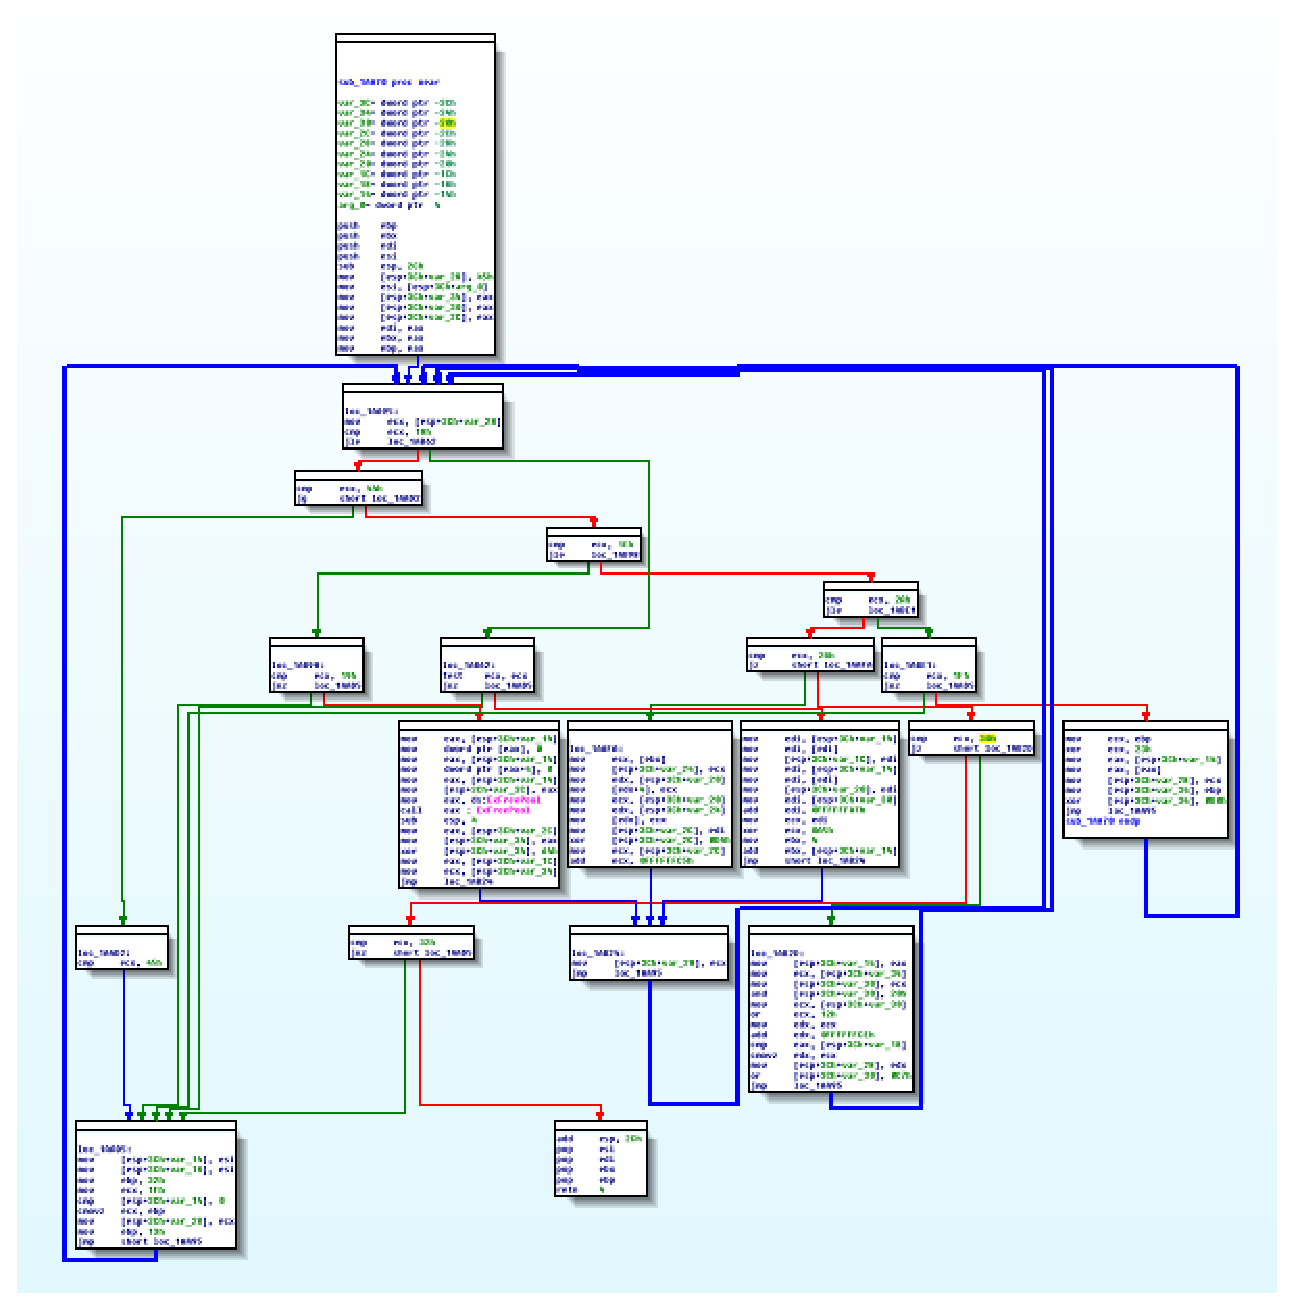
\includegraphics[height=0.8\textheight]{figs/mebroot_obf_01.eps}
    \end{center}
  \end{figure}
\end{frame}



\tikzset{bloc/.style={
    rectangle,minimum size=6mm, minimum width=6em,
    very thick,draw=black!50,
    top color=white,bottom color=black!20,
    rounded corners,
    font=\scriptsize}}


\tikzset{mywave/.style={
    snake=expanding waves,segment length=2mm, segment angle=20}}

\begin{frame}

\begin{columns}

\column{0.4\textwidth}

\begin{bigcenter}
\begin{figure}
\scalebox{0.5}{
\begin{tikzpicture}[node distance = 3cm,>=latex']
  \node [bloc] (b1)   {b1};
  \node [bloc, below right of=b1] (b2)   {b2};
  \node [bloc, below left of=b1] (b3)   {b3};
  \node [bloc, below left of=b2] (b4)   {b4};

  \draw[->] (b1) -- (b2);
  \draw[->] (b1) -- (b3);
  \draw[->] (b2) -- (b4);
  \draw[->] (b3) -- (b4);

\end{tikzpicture}
}
\end{figure}
\end{bigcenter}
\column{0.4\textwidth}
\begin{bigcenter}
\scalebox{0.5}{
\begin{tikzpicture}[node distance = 3cm,>=latex']
  \node [bloc] (b0)   {\begin{minipage}{2cm}\begin{center}b0\\e = 0\end{center}\end{minipage}};


  \node [bloc, below of=b0] (dispatch)   {dispatcher};


  \node [bloc, below left of=dispatch] (b2)   {\begin{minipage}{2cm}\begin{center}b2\\e = 4\end{center}\end{minipage}};
  \node [bloc, left of=b2] (b1)   {\begin{minipage}{2cm}\begin{center}b1\\e = [2,3]\end{center}\end{minipage}};
  \node [bloc, below right of=dispatch] (b3)   {\begin{minipage}{2cm}\begin{center}b3\\e = 4\end{center}\end{minipage}};
  \node [bloc, right of=b3] (b4)   {\begin{minipage}{2cm}\begin{center}b3\\e = ?\end{center}\end{minipage}};


  \draw[->] (b0) -- (dispatch);
  \draw[->] (dispatch) -- (b1);
  \draw[->] (dispatch) -- (b2);
  \draw[->] (dispatch) -- (b3);
  \draw[->] (dispatch) -- (b4);

  \draw[->] (b1) to [out = 135, in=180] (dispatch);
  \draw[->] (b2) to [out = 135, in=180] (dispatch);
  \draw[->] (b3) to [out = 45, in=0] (dispatch);
  \draw[->] (b4) to [out = 45, in=0] (dispatch);



\end{tikzpicture}
}
\end{bigcenter}
\end{columns}
\end{frame}

\begin{frame}
  \begin{block}{Reconstruction}
    \begin{itemize}
      \item disassemble a function
      \item get semantic of each bloc
      \item symbolic execution
      \item get each bloc result of the automata
      \item patch jcc
      \item regenerate binary
    \end{itemize}
  \end{block}
\end{frame}

\begin{frame}
  \frametitle{R�sultat}
  \begin{figure}[htp]
    \begin{center}
      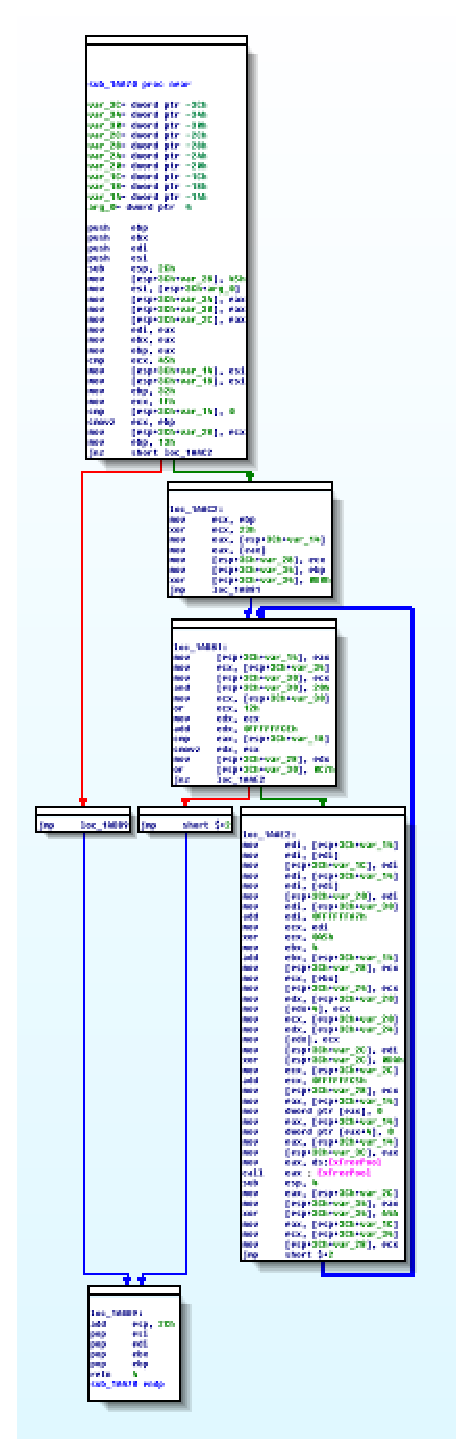
\includegraphics[height=0.8\textheight]{figs/mebroot_obfdel_01.eps}
    \end{center}
  \end{figure}
\end{frame}



\subsection{VM Study}

\begin{frame}
  \frametitle{first layer}
  \begin{block}{Packer}
    \begin{itemize}
      \item The binary is ciphered by layers.
      \item Just create an environment and emulate it with miasm.
    \end{itemize}
  \end{block}
  \begin{center}
    \includegraphics[width=0.7\textwidth]{figs/xxx_vm01.eps}
  \end{center}
\end{frame}


\begin{frame}
  \frametitle{First disassembling of vm mnemonic parsing}
  \begin{center}
    \includegraphics[width=0.7\textwidth]{figs/xxx_mnemo02.eps}
  \end{center}
\end{frame}

\begin{frame}
  \frametitle{Obfuscation}
  \begin{center}
    \includegraphics[width=1.0\textwidth]{figs/xxx_mnemo03.eps}
  \end{center}
\end{frame}

\begin{frame}
  \begin{block}{Solution}
    \begin{itemize}
      \item Callback is the disassembler engine
      \item symbolic execution of its parents
      \item Test if jcc is always true/false
      \item and delete fake edges
    \end{itemize}
  \end{block}
  
\end{frame}

\begin{frame}
  \frametitle{Result: simplified mnemonic parser}
\begin{tabular}{p{5cm} p{5cm} }
    \includegraphics[width=0.08\textwidth]{figs/xxx_mnemo08.eps}
 &
    \includegraphics[width=0.13\textwidth]{figs/xxx_mnemo09.eps}
\end{tabular}

\end{frame}

\begin{frame}
  \frametitle{End of parser: instruction dispatcher}
  \begin{center}
    \includegraphics[width=0.8\textwidth]{figs/xxx_mnemo10.eps}
  \end{center}
\end{frame}


\begin{frame}[fragile]
  \begin{exampleblock}{symbolic execution: touched variables}
    {\tiny\begin{semiverbatim}
eax = ((((@8[init_esi] ^ init_ebx[0:8]) - 0xA8) ^ 0x1)_to[0:8], 0x0_to[8:32])
ebx = ((init_ebx[0:8] - (((@8[init_esi] ^ init_ebx[0:8]) - 0xA8) ^ 0x1))_to[0:8], init_ebx[8:32]_to[8:32])
esi = (init_esi + 0x1)
DST @32[((((((@8[init_esi] ^ init_ebx[0:8]) - 0xA8) ^ 0x1)_to[0:8], 0x0_to[8:32]) * 0x4) + init_edi)]
    \end{semiverbatim}}
  \end{exampleblock}
  \begin{block}{Note}
    \begin{itemize}
    \item We need to follow modifications of ebx, esi, edi in each vm mnemonic
    \item Those modifications are needed to known where disassembling next mnemonic
    \end{itemize}
  \end{block}
\end{frame}

\begin{frame}
  \frametitle{Disassembling correction}
  \begin{center}
    \includegraphics[width=0.8\textwidth]{figs/xxx_mnemo04.eps}
  \end{center}
\end{frame}

\begin{frame}
  \frametitle{Bloc grouping}
  \begin{center}
    \includegraphics[width=1.0\textwidth]{figs/xxx_mnemo05.eps}
  \end{center}
\end{frame}

\begin{frame}
  \frametitle{More than 150 vm mnemonic}
  \begin{center}
    \includegraphics[width=1.0\textwidth]{figs/xxx_mnemo07.eps}
  \end{center}
\end{frame}

\begin{frame}
  \frametitle{Bloc analysis: erf}
  \begin{center}
    \includegraphics[width=0.6\textwidth]{figs/xxx_mnemo06.eps}
  \end{center}
\end{frame}


\begin{frame}[fragile]
  \frametitle{But symbolic execution (again :p)}
{\tiny\begin{semiverbatim}
Registers after a bloc execution
 eax init_eax  
 ebx init_ebx  
 ecx (@16[init_esp]_to[0:16], init_ecx[16:32]_to[16:32])  
 edx init_edx  
 esi init_esi  
 edi init_edi  
 esp (init_esp-0x2)  
 ebp init_ebp  

stack modification:
 @16[(init_esp+0x2)]    (@16[(init_esp+0x2)]<<(@8[init_esp]&0x1F))
 @32[(init_esp-0x2)]    ((@8[init_esp]&0x1F)?(0x0,((@16[(init_esp+0x2)]>>(0x10-(@8[init_esp]&0x1F)))&0x1))_to[0:1], 0x1_to[1:2], (parity (@16[(init_esp+0x2)]<<(@8[init_esp]&0x1F)))_to[2:3], 0x0_to[3:4], (((init_esp+0x2)&0x10)==0x10)_to[4:5], 0x0_to[5:6], ((@16[(init_esp+0x2)]<<(@8[init_esp]&0x1F))==0x0)_to[6:7], ((0x1==((@16[(init_esp+0x2)]<<(@8[init_esp]&0x1F))>>0xF))&0x1)_to[7:8], 0x2_to[8:11], ((0x1==((@16[(init_esp+0x2)]<<(@8[init_esp]&0x1F))>>0xF))^((@16[(init_esp+0x2)]>>(0x10-(@8[init_esp]&0x1F)))&0x1))_to[11:12], 0x0_to[12:32])
 
Result:
\textcolor{blue}{a = pop16
b = pop16
push16(a<<b)
push32(eflag)}      
  \end{semiverbatim}}
\end{frame}


\begin{frame}[fragile]
  \frametitle{Another example}
{\tiny\begin{semiverbatim}
---------- 12 0x6fab03 ----------
eax = @32[init_esp]
@32[(init_esp+0x4)]    (@32[(init_esp+0x4)]-@32[init_esp])
@32[init_esp]    (flags(@32[(init_esp+0x4)]-@32[init_esp]))
---------- 13 0x6fb100 ----------
eax = @32[init_esp]
esp = (init_esp+0x4)
@32[(init_esp+0x4)]    (@32[(init_esp+0x4)]^@32[init_esp])
---------- 15 0x6fb3b2 ----------
@32[(init_edi+0x1C)]    (@32[(init_edi+0x1C)]&0xFFFFFBFF)
---------- 19 0x6fb6b8 ----------
ecx = @32[init_esp]
esp = (init_esp+0x4)
@32[(init_esp+0x4)]    (@32[(init_esp+0x4)]<<(@8[init_esp]&0x1F))
---------- 21 0x6fb97e ----------
eax = @32[init_esp]
@32[init_esp]    @32[@32[init_esp]]
---------- 24 0x6fc3d1 ----------
eax = ((((@16[init_esi]_to[0:16], init_eax[16:32]_to[16:32])+init_ebx)^0x18EE5784)-0x12C0A81E)
ebx = (init_ebx^((((@16[init_esi]_to[0:16], init_eax[16:32]_to[16:32])+init_ebx)^0x18EE5784)-0x12C0A81E))
edx = (init_edx^((((@16[init_esi]_to[0:16], init_eax[16:32]_to[16:32])+init_ebx)^0x18EE5784)-0x12C0A81E))
esi = (init_esi+0x2)
---------- 28 0x6fc935 ----------
...
esp = (init_esp-0x4)
@32[(init_esp+0x4)]    (@32[(init_esp+0x4)] umul32_hi @32[init_esp])
@32[init_esp]    (@32[(init_esp+0x4)] umul32_lo @32[init_esp])
@32[(init_esp-0x4)]    (0x2_to[0:2], (parity init_edi)_to[2:3], 0x0_to[3:4], (((init_esp+0x4)&0x10)==0x10)_to[4:5], 0x0_to[5:6], (init_edi==0x0)_to[6:7], ((0x1==(init_edi>>0x1F))&0x1)_to[7:8], 0x2_to[8:32])
  \end{semiverbatim}}
\end{frame}

\begin{frame}[fragile]
  \begin{block}{Instruct the interpreter}
    \begin{itemize}
    \item \verb?@32[(init_edi+0x1C)]? is the vm eflagest le eflag de la vm
    \item we replace \verb?@8[(init_edi+0x28)]?, by  REG1, REG2, ...
    \item we replace \verb?esp+X? by registers \verb?arg32_0?,  ...
    \end{itemize}
  \end{block}
\end{frame}

\begin{frame}[fragile]
  \frametitle{Instruction}
  \lstset{language=Python}
	 {\tiny\begin{lstlisting}[]{}  
known_vm_e = {
    init_edi + ExprInt(uint32(0x1C)): regflag,
    init_edi + ExprInt(uint32(0x20)): reg1,
    init_edi + ExprInt(uint32(0x24)): reg2,
    init_edi + ExprInt(uint32(0x28)): reg3,
    init_edi + ExprInt(uint32(0x2C)): reg4,
    init_edi + ExprInt(uint32(0x30)): reg5,
    init_edi + ExprInt(uint32(0x34)): reg6,
    init_edi + ExprInt(uint32(0x38)): reg7,
    init_edi + ExprInt(uint32(0x3C)): reg8,
    init_edi + ExprInt(uint32(0x40)): reg9,

    ExprMem(init_esp-ExprInt(uint32(4))): argm1_32,
    ExprMem(init_esp-ExprInt(uint32(2))): argm1_16,
    ExprMem(init_esp): arg0_32,
    ExprMem(init_esp+ExprInt(uint32(4))): arg1_32,
    ExprMem(init_esp, size = 16): arg0_16,
    ExprMem(init_esp+ExprInt(uint32(2)), size=16): arg1_16,
    ExprMem(init_esp, size = 8): arg0_08,
    ExprMem(init_esp+ExprInt(uint32(4)), size=8): arg1_08,
}
	 \end{lstlisting}}
\end{frame}

\begin{frame}[fragile]
  \frametitle{Results}
{\tiny\begin{semiverbatim}
---------- 143 0x70a4f5 ----------    
esp = (init_esp - 0x4)                
arg-1_32 = @32[init_edx]              
\textcolor{blue}{=> push 32@[edx]}
---------- 151 0x70b1e1 ----------
eax = arg1_32
ecx = (arg1_32_to[0:8], ((0x1 == (arg1_08 >> 0x7)) == 0x1)?(0x0,0xFFFFFFFF)_to[8:32])
esp = (init_esp + 0x4)
arg1_32 = (arg1_32_to[0:8], ((0x1 == (arg1_08 >> 0x7)) == 0x1)?(0x0,0xFFFFFFFF)_to[8:32])
\textcolor{blue}{=> pop   dum
   pop   X
   movsx X, X8
   push  X}
---------- 154 0x70b8b4 ----------
ecx = (arg0_16_to[0:16], init_ecx[16:32]_to[16:32])
esp = (init_esp - 0x2)
arg1_16 = (arg1_16 a>> (arg0_08 & 0x1F))
arg-1_16 = ... flags of op ...
\textcolor{blue}{=> push arg1_16 >> arg0_08
   push eflags}
---------- 158 0x70bb56 ----------
esp = (init_esp - 0x4)
arg-1_32 = @32[reg4]
\textcolor{blue}{=> push @32[reg4]}
---------- 155 0x70ba09 ----------
arg0_32 = (! arg0_32)
DST 0x6F88F1
\textcolor{blue}{=> not @32[esp]}
  \end{semiverbatim}}
\end{frame}

\begin{frame}
  \begin{block}{Multi bloc mnemonic}
    \begin{itemize}
    \item A mnemonic can have a complex graph
    \item we can evaluate a bloc, and propagate its state to its sons
    \item and so on
    \item No loop for the moment
    \end{itemize}
  \end{block}
\end{frame}

\begin{frame}[fragile]
  \frametitle{Result: multiple vm exit}
\begin{tabular}{p{5cm} p{5cm}}
\multicolumn{2}{c}{ teste si reg7 == 0x0}
\\      
{\tiny\begin{semiverbatim}

\textcolor{blue}{---------- state 1 ----------}
eax = @32[(init_esp + 0x1C)]
ebx = @32[(init_esp + 0x10)]
ecx = @32[(init_esp + 0x18)]
edx = @32[(init_esp + 0x14)]
esi = arg1_32
edi = arg0_32
\textcolor{blue}{the vm does not unstack args}
esp = (init_esp + 0x28)
ebp = @32[(init_esp + 0x8)]
@32[reg5] = 0x0
DST @32[(init_esp + 0x24)]
  \end{semiverbatim}}
&
{\tiny\begin{semiverbatim}
\textcolor{blue}{---------- state 2 ----------}
eax = @32[(init_esp + 0x1C)]
ebx = @32[(init_esp + 0x10)]
ecx = @32[(init_esp + 0x18)]
edx = @32[(init_esp + 0x14)]
esi = arg1_32
edi = arg0_32
\textcolor{blue}{the vm unstack reg7 arguments}
esp = ((init_esp + @32[reg7]) + 0x28)
ebp = @32[(init_esp + 0x8)]
@32[reg7] = 0x0
@32[reg5] = 0x0
arg-1_32 = ((init_esp + @32[reg7]) + 0x24)
DST @32[(init_esp + 0x24)]
  \end{semiverbatim}}
\end{tabular}
\end{frame}

\end{document}


